%%%% fatec-article.tex, 2024/03/10

%% Classe de documento
\documentclass[
landscape,
  a4paper,%% Tamanho de papel: a4paper, letterpaper (^), etc.
  12pt,%% Tamanho de fonte: 10pt (^), 11pt, 12pt, etc.
  english,%% Idioma secundário (penúltimo) (>)
  brazilian,%% Idioma primário (último) (>)
]{article}

%% Pacotes utilizados
\usepackage[]{fatec-article}
\usepackage{setspace}

%% Processamento de entradas (itens) do índice remissivo (makeindex)
%\makeindex%

%% Arquivo(s) de referências
%\addbibresource{fatec-article.bib}

%% Início do documento
\begin{document}

% Seções e subseções
%\section{Título de Seção Primária}%

%\subsection{Título de Seção Secundária}%

%\subsubsection{Título de Seção Terciária}%

%\paragraph{Título de seção quaternária}%

%\subparagraph{Título de seção quinária}%

%\section*{Diário de Bordo}%
\section*{Instruções para o preenchimento}
\doublespacing
\begin{enumerate}
    \item O Diário de Bordo é usado para registrar atividades, progressos, ideias e desafios enfrentados em um projeto ou durante a rotina de trabalho. Serve como um registro cronológico e detalhado das operações diárias, facilitando a organização e o acompanhamento das tarefas.
    \doublespacing
    \item Durante o registro das atividades deve-se incluir detalhes como datas, horários, descrições de tarefas, nomes de participantes e observações relevantes.  Esta documentação contínua ajuda na avaliação do progresso de projetos ou atividades, permitindo ajustes e melhorias contínuas nos processos.
    \doublespacing
    \item Para evidenciar a realização das tarefas, você poderá utilizar a criação de anexos para adicionar anotações, fotos, prints, questionários, entre outros.
\end{enumerate}

\break


\begin{table}[]
  \centering
  \begin{tabular}{|l|l|l|l|l|}
  \hline
  Nome da Atividade & Data de início & Data de término & Responsável pela atividade & Descrição da atividade realizada \\ \hline
                    Definição de objetivos              &17/02/2025&17/02/2025  &Ricardo e Valmir &Definição de Objetivos para 6º semestre\\ \hline
                    Orientação para correção do artigo     &07/04/2025&02/05/2025  &Ricardo e Valmir &Refatoração do artigo\\ \hline
                    Adição da equipe ao protótipo figma &07/04/2025&02/05/2025  &Vinicius e Derick           &Correção do Artigo\\ \hline
                    Novo Protótipo                      &05/05/2025&12/05/2025  &Derick e Vinicius           &Ajuste de telas\\ \hline
                    Artigo Científico                   &05/05/2025&12/05/2025  &Ricardo e Valmir         &Revisão e resumo \\\hline

                    &                            &                &                 &                                  \\ \hline
                    &                            &                &                 &                                  \\ \hline
                    &                            &                &                 &                                  \\ \hline
                    &                            &                &                 &                                  \\ \hline
                    &                            &                &                 &                                  \\ \hline
                    &                            &                &                 &                                  \\ \hline
                    &                            &                &                 &                                  \\ \hline
                    &                            &                &                 &                                  \\ \hline
  \end{tabular}
  \end{table}

\begin{figure}
  \centering
  \caption{Desenvolvimento Mobile}
  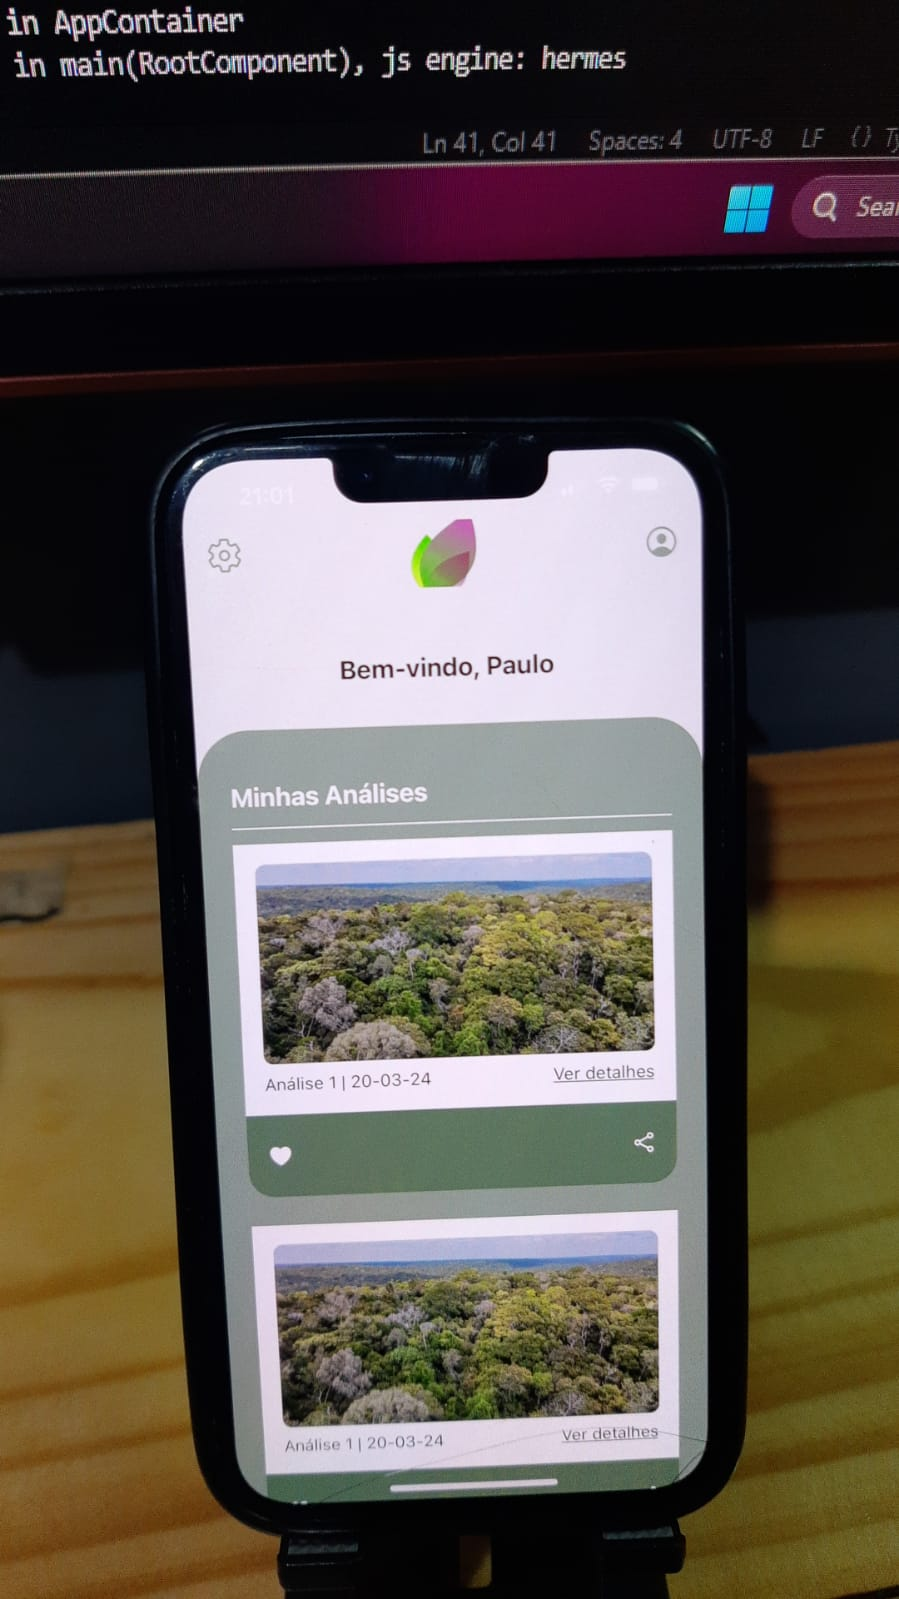
\includegraphics[width=.3\textwidth,keepaspectratio]{Logos/mobile01.jpeg}
  \SourceOrNote{Fonte: Os Autores(2025)}
  \label{fig:enter-label}
\end{figure}




\end{document}